\documentclass[11pt,a4paper]{article}

\usepackage[utf8]{inputenc}
\usepackage[T1]{fontenc}
\usepackage{lmodern}
\usepackage{microtype}
\usepackage[margin=2.5cm]{geometry}
\usepackage{booktabs}
\usepackage{array}
\usepackage{graphicx}
\usepackage{amsmath}
\usepackage[dvipsnames]{xcolor}
\usepackage{tikz}
\usetikzlibrary{arrows.meta,calc}
\usepackage{float}
\usepackage{etoolbox}
\usepackage{fancyhdr}
\usepackage{tocloft}
\setlength{\cftbeforesecskip}{4pt}
\setlength{\cftbeforesubsecskip}{0pt}
\setlength{\cftbeforefigskip}{4pt}
\setlength{\cftbeforetabskip}{3pt}
\usepackage{enumitem}
\usepackage[font=small,labelfont=bf]{caption}
\usepackage[numbers]{natbib}
\usepackage[colorlinks=true,linkcolor=blue!50!black,citecolor=blue!50!black,urlcolor=blue!50!black,
  hypertexnames=false,pdfpagelabels,pdftitle={LeakScope: Auditing What Information Was Actually Available at Prediction Time},
  pdfauthor={Aissati Oussama}]{hyperref}
\usepackage[all]{hypcap}

\graphicspath{{../assets/}}
\definecolor{navy}{HTML}{14213D}
\definecolor{teal}{HTML}{1F7A8C}
\definecolor{leakred}{HTML}{C8553D}
\definecolor{okgreen}{HTML}{2A9D8F}
\definecolor{softgray}{HTML}{F2F4F7}
\newcommand{\statbox}[4]{%
  \node[draw=teal,fill=softgray,rounded corners=3pt,minimum width=3.75cm,minimum height=2.1cm,
        align=center,font=\sffamily,inner sep=4pt,text width=3.4cm]
    at ([xshift=#1,yshift=-21.2cm]current page.north west)
    {{\Large\bfseries\textcolor{navy}{#2}}\\[2pt]{\footnotesize\textcolor{gray!70!black}{#3}}};}
\renewcommand{\subsectionautorefname}{Section}
\renewcommand{\sectionautorefname}{Section}
\pagestyle{fancy}\fancyhf{}
\fancyhead[R]{\small\textcolor{gray}{LeakScope}}
\fancyfoot[C]{\thepage}
\renewcommand{\headrulewidth}{0.3pt}
\setlength{\parskip}{0.4em}
\setlist{itemsep=0.2em,topsep=0.3em}

% feature and command names: monospaced, underscores allowed
\newcommand{\ft}[1]{\texttt{\detokenize{#1}}}
\newcommand{\tpred}{$t_{\mathrm{pred}}$}

\begin{document}
\pagenumbering{roman}

%%%%%%%%%%%%%%%%%%%% TITLE PAGE %%%%%%%%%%%%%%%%%%%%
\begin{titlepage}
\thispagestyle{empty}
\begin{tikzpicture}[remember picture,overlay]
  % header band
  \fill[navy] (current page.north west) rectangle ([yshift=-9.4cm]current page.north east);
  \fill[teal] ([yshift=-9.4cm]current page.north west) rectangle ([yshift=-9.65cm]current page.north east);
  \node[anchor=north west,text=white,font=\sffamily\small\bfseries,text width=16cm]
    at ([xshift=2.5cm,yshift=-2.4cm]current page.north west) {TECHNICAL REPORT \quad|\quad TEMPORAL DATA LEAKAGE};
  \node[anchor=north west,text=white,font=\sffamily\fontsize{40}{44}\selectfont\bfseries,text width=16cm]
    at ([xshift=2.5cm,yshift=-3.8cm]current page.north west) {LeakScope};
  \node[anchor=north west,text=white,font=\sffamily\Large,text width=15.5cm]
    at ([xshift=2.5cm,yshift=-6.0cm]current page.north west)
    {Auditing what information was actually available at prediction time};
  \node[anchor=north west,text=white!80!navy,font=\sffamily\normalsize,text width=15.5cm]
    at ([xshift=2.5cm,yshift=-7.9cm]current page.north west)
    {A temporal data-leakage auditor, with a controlled study of what leaks do to a model's score};

  % timeline
  \begin{scope}[shift={([xshift=10.5cm,yshift=-15.6cm]current page.north west)},font=\sffamily\footnotesize]
    \fill[okgreen!14] (-8,-0.9) rectangle (0,0.9);
    \fill[leakred!14] (0,-0.9) rectangle (8.2,0.9);
    \draw[-{Stealth[length=2.5mm]},thick,navy] (-8,0) -- (8.5,0) node[right=2pt] {time};
    \draw[dashed,thick,navy] (0,-1.1) -- (0,1.5);
    \node[navy,font=\sffamily\small\bfseries,above=1pt] at (0,1.5) {$t_{\mathrm{pred}}$ (pickup: the prediction is made)};
    \node[okgreen!60!black,font=\sffamily\footnotesize\bfseries] at (-4,0.55) {usable at $t_{\mathrm{pred}}$};
    \node[leakred,font=\sffamily\footnotesize\bfseries] at (4.1,0.55) {not yet available: a leak};
    \foreach \x/\lab in {-6.6/{earlier trips\\finished}, -3.2/{zone averages\\computed}, -1.0/{pickup fields\\known}}{
      \fill[okgreen] (\x,0) circle (0.13);
      \node[text width=2.4cm,align=center,text=okgreen!60!black,below=4pt] at (\x,0) {\lab};}
    \foreach \x/\lab in {2.4/{dropoff: trip ends\\(event time, R1)}, 4.9/{fare recorded +2 min\\(availability, R2)}, 7.3/{fare corrected\\next day 06:00 (R2)}}{
      \fill[leakred] (\x,0) circle (0.13);
      \node[text width=2.5cm,align=center,text=leakred,below=4pt] at (\x,0) {\lab};}
  \end{scope}

  % key figures
  \statbox{3.9cm}{4}{rules R1 to R4}{}
  \statbox{8.3cm}{15}{labelled scenarios}{}
  \statbox{12.7cm}{19}{features audited}{}
  \statbox{17.1cm}{100\,000}{prediction examples}{}

  % author block
  \draw[teal,thick] ([xshift=2.5cm,yshift=-24.2cm]current page.north west) -- ([xshift=-2.5cm,yshift=-24.2cm]current page.north east);
  \node[anchor=north west,font=\sffamily\Large\bfseries,text=navy]
    at ([xshift=2.5cm,yshift=-24.9cm]current page.north west) {Aissati Oussama};
  \node[anchor=north west,font=\sffamily\normalsize,text=navy,text width=16cm]
    at ([xshift=2.5cm,yshift=-25.9cm]current page.north west)
    {\href{https://github.com/0utc/leakscope}{github.com/0utc/leakscope}\\[3pt] November 2026};
  \node[anchor=north east,font=\sffamily\footnotesize,text=gray!70!black,text width=7cm,align=right]
    at ([xshift=-2.5cm,yshift=-25.0cm]current page.north east)
    {Case study: NYC yellow-taxi trips, January 2024\\Python \textperiodcentered{} DuckDB \textperiodcentered{} scikit-learn};
\end{tikzpicture}
\end{titlepage}

%%%%%%%%%%%%%%%%%%%% FRONT MATTER %%%%%%%%%%%%%%%%%%%%
\begin{abstract}
\noindent
A model that predicts the future must only use information that existed at the moment of prediction. Features that break this rule inflate offline scores and then fail in production. This report presents LeakScope, a small auditor in which every feature declares when the underlying event happened, when its value became usable, and, for aggregates, exactly which rows it covers. Four rules check these declarations against the prediction time, and a conformance check recomputes stored aggregates by brute force to catch declarations that lie. The auditor is tested on 15 labelled scenarios (10 leaky, 5 valid) built on NYC yellow-taxi trips (January 2024; 100{,}000 prediction examples; target: trip duration at pickup). It flags all 10 leaky and none of the 9 valid features, but the scenarios were designed together with the auditor, so this shows agreement with the specification, not general detection power. A controlled comparison then adds each leak to an honest model. Offline, a model with all leaks reaches an MAE of 1.451 min, 78.7\% below the honest model (6.817 min); when the leaked values are unavailable at serving time, the same model scores 8.471 min, 24.3\% \emph{worse} than the honest model. The share of rows flagged by the auditor does not predict the damage: seven leaky features are flagged on 100\% of rows, yet their offline effect ranges from $-0.3\%$ to $-68.4\%$. Two further sources of uncertainty are quantified (test-set sampling and float-level feature noise, the latter moving a model's MAE by up to 0.066 min), and a third, covering other splits, months and model seeds, is explicitly not studied. All availability times are simulated; the report states what that does and does not support.
\end{abstract}

\vspace{1.2em}
\noindent\textbf{At a glance}
\begin{center}
\small
\renewcommand{\arraystretch}{1.25}
\begin{tabular}{@{}p{5.2cm}p{9.6cm}@{}}
\toprule
Audit & 10 of 10 leaky features flagged; 9 of 9 valid features left alone (scenarios co-designed with the auditor) \\
Honest model & MAE 6.817 min on the test week (constant-median baseline: 7.787) \\
All leaks, offline & MAE 1.451 min, $-78.7\%$ vs the honest model \\
Same model, leaks unavailable & MAE 8.471 min, $+24.3\%$ vs the honest model \\
Float-noise jitter & up to 0.066 min in one model's MAE; quote 6.817 min (SD 0.007) \\
Not studied & other splits, months, model seeds; real (not simulated) availability lags \\
\bottomrule
\end{tabular}
\end{center}

\clearpage
\tableofcontents
\clearpage
\listoffigures
\vspace{2em}
\listoftables
\clearpage
\pagenumbering{arabic}

\section{Introduction}
Leakage is the use of information about the prediction target that would not legitimately be available when the model is used. It is a well-known cause of over-optimistic results: Kaufman et al.\ define it as the introduction of information about the target that should not be available to mine from, and argue that avoiding it requires an explicit account of what the model is supposed to know and when~\cite{kaufman2012}. Kapoor and Narayanan survey prior reviews and find leakage affecting at least 294 papers across 17 scientific fields, and propose a taxonomy of eight leakage types~\cite{kapoor2023}.

Much leakage is \emph{temporal}: a value is used that did not yet exist, or existed but was not yet usable, at prediction time. Such leaks are easy to introduce and hard to see in a score. A joined table may be correct on average yet wrong for each row; an aggregate may include the row it is predicting; a snapshot may be taken at the end of the day. Checking only the final metric does not reveal them, as this report shows.

\paragraph{What this project does.} LeakScope makes the temporal assumptions of a feature pipeline explicit and checkable. Every feature declares an \emph{event time} (when the underlying thing happened), an \emph{availability time} (when a serving system could use it), and whether it is known only after the outcome. Four rules evaluate these declarations against the prediction time \tpred{} for every example. A conformance check then verifies that stored aggregate values really follow their declared definition. A controlled machine-learning experiment measures what each leak does to a model's offline and production-condition score.

\paragraph{Contributions, stated modestly.}
\begin{itemize}
  \item A declarative feature registry and four rules (R1--R4) that detect future events, late availability, declared post-outcome fields and incorrect aggregation, with explanations naming a concrete example.
  \item A conformance check that recomputes aggregates from their declaration, which closes a gap the declaration-based rules cannot see (a false declaration).
  \item A labelled benchmark of 15 scenarios, including exact-boundary cases (available at exactly \tpred{} is valid; one second later is not).
  \item A controlled study that adds each leak to an honest model, with paired block-bootstrap intervals, production-condition scoring, ablations, and a float-noise sensitivity analysis.
  \item An open, reproducible implementation: one command runs everything on synthetic data, and the results here come from the real data with fixed seeds.
\end{itemize}

\paragraph{What this project does not claim.} It does not claim to detect all leakage. The scenarios and the auditor were designed together, availability times are simulated, and the experiments use one month of data, one split and one model class. \autoref{sec:limits} lists the limits in full.

\section{Related Work}
\textbf{Leakage in machine learning.} Kaufman et al.~\cite{kaufman2012} give a formal treatment of leakage, a methodology for avoiding it (a ``learn-predict separation'' at the data-management level) and ways to detect it when the modeller does not control data collection. Kapoor and Narayanan~\cite{kapoor2023} document how widespread leakage is in ML-based science and introduce ``model info sheets'' as a reporting tool. LeakScope is narrower than both: it targets one family, temporal availability, in tabular prediction pipelines, and turns the question ``was this usable at \tpred{}?'' into a rule that can be run.

\textbf{Evaluation under time dependence.} How to split time-dependent data is itself a design choice. Bergmeir and Benítez compare cross-validation variants with last-block evaluation for time-series predictors; they found no practical consequence of the theoretical objections to cross-validation in their study, and recommended blocked cross-validation~\cite{bergmeir2012}. This project uses the simplest option, a single chronological split, and adds \emph{purging}: training examples whose label was not yet available at the cutoff are excluded, so no training label comes from the future (\autoref{sec:split}).

\textbf{Uncertainty for dependent data.} Trips in the same hour share traffic conditions, so resampling single rows would give intervals that are too narrow. Block resampling for dependent observations goes back to K\"unsch~\cite{kunsch1989}, and the bootstrap itself to Efron~\cite{efron1979}. The analysis here resamples whole hours of the test week.

\textbf{Tooling.} The pipeline runs on DuckDB~\cite{raasveldt2019} and the model is scikit-learn's histogram-based gradient boosting~\cite{pedregosa2011}. Point-in-time correct joins are standard practice in feature-serving systems; a comparison with such a system is future work (\autoref{sec:future}) and is not claimed here.

\section{Method}
\subsection{Event time, availability time and the core rule}
\emph{Event time} is when something happened in the real world. \emph{Availability time} is when the information becomes usable by a prediction service. The two differ: a taxi trip ends at its dropoff, but its fare may be recorded minutes later and corrected the next day. The core rule is:
\begin{equation}
  \text{a feature value may be used for a prediction at } t_{\mathrm{pred}} \iff \text{availability time} \le t_{\mathrm{pred}}.
\end{equation}
The comparison is inclusive: a value available at exactly \tpred{} is valid, and a value available one second later is not. Both cases are tested explicitly (scenarios N4 and L10).

\subsection{Feature registry}
Each feature is described in a YAML registry with its source, a transformation text, its event clock, its availability clock, a flag \ft{declared_post_outcome}, and whether it is a \ft{row} feature or an \ft{aggregate}. Aggregates additionally declare their grouping (\ft{pu_zone}), their window (\ft{whole_dataset}, \ft{up_to_t_pred} or \ft{lookback} with a length), the clock the window is defined on (\ft{avail_dropoff} or \ft{event_pickup}) and \ft{includes_current_row}. The registry is validated on load; an invalid registry fails with a list of every problem. Row features may use the example's own trip as their source or a \emph{looked-up} trip recorded in a lineage table (needed for L9, whose value comes from a different trip).

\subsection{The four rules}
\autoref{tab:rules} defines the four rules; each is evaluated for every prediction example.
\begin{table}[H]
\centering\small
\caption{The four audit rules R1 to R4.}
\label{tab:rules}
\begin{tabular}{@{}lp{11.5cm}@{}}
\toprule
Rule & Fires when \\
\midrule
R1 & the feature's event time is after \tpred{} (it describes something that had not yet happened) \\
R2 & the feature's availability time is after \tpred{} (it had happened but was not yet usable) \\
R3 & the feature is declared to be known only after the outcome \\
R4 & an aggregate uses source rows that are not yet available at \tpred{}, including the example's own row \\
\bottomrule
\end{tabular}
\end{table}
As \autoref{tab:rules} states, R1 and R2 are evaluated per example against the clocks of the record the feature was built from. When metadata is consistent, R1 implies R2, so R1 is the stronger diagnosis. R3 catches metadata that lies about both clocks: a feature declared post-outcome is invalid whatever its timestamps say (scenario L1). R4 counts, for every example, the source trips an aggregate uses that were not available at \tpred{}: a whole-dataset window counts every later trip; an availability-clock window can only be violated by the example's own trip; a pickup-clock window counts trips still in progress, which is computed with a bucket join (bucket width equal to the window length, so a window spans at most two buckets) to avoid scanning tens of thousands of trips per example. Every finding reports the number of violating examples, the share, a few trip IDs, and a plain-language explanation with one worked example.

\subsection{Conformance check}
R4 judges the \emph{declaration} of an aggregate. If the declaration is false, for instance it says ``availability-based window'' while the stored values were built from a pickup-time window, R1--R4 see nothing wrong. The conformance check closes this loop: for a deterministic sample of 30 examples it recomputes the aggregate by brute force from the declaration and compares it with the stored value (relative tolerance $10^{-6}$). A fixture with a deliberately lying aggregate (known limitation M1) is missed by all four rules and caught by the check (5 mismatching examples). The check covers six stored aggregates; any aggregate outside this list is not covered.

\subsection{Point-in-time retrieval}
Historical statistics are computed only from trips whose simulated availability time is at most \tpred{}. Running totals of duration are kept per zone, ordered by availability time. An ASOF join finds, for each example, the last running-total row at or before \tpred{}; a lookback average over $(t_{\mathrm{pred}}-L, t_{\mathrm{pred}}]$ is the difference between the running totals at \tpred{} and at $t_{\mathrm{pred}}-L$. The window is left-open and right-closed, and an example without history gets a missing value rather than zero. Durations are accumulated as integer seconds: summing decimal minutes in window functions was found to be order-dependent for tied timestamps and made rebuilds differ at the $10^{-13}$ level (\autoref{sec:defect}).

\subsection{Labelled scenarios}
\autoref{tab:scen} lists the 15 scenarios; each has a ground-truth set of rules it must trigger, written before the auditor was built. A scenario may trigger several rules. N4 and L10 run on a tiny in-memory fixture, the others on the taxi data.

\begin{table}[H]
\centering\small
\caption{Labelled scenarios and the rules each must trigger.}
\label{tab:scen}
\begin{tabular}{@{}l p{8.6cm} l@{}}
\toprule
ID & Scenario & Expected \\
\midrule
L1 & Final trip distance; the registry wrongly claims it was recorded at pickup & R3 \\
L2 & Final total fare of the trip itself & R1, R2 \\
L3 & Dropoff hour of the trip itself & R1, R2, R3 \\
L4 & Zone average over the whole dataset (future trips and the own trip) & R4 \\
L5 & 60-minute zone average that includes the example's own trip & R4 \\
L6 & 60-minute zone average by pickup time, including trips in progress & R4 \\
L7 & Next-day corrected fare of the trip itself & R1, R2 \\
L8 & Zone average snapshot taken at the end of the prediction day & R1, R2 \\
L9 & Fare of the last completed zone trip looked up by dropoff time instead of fare availability time & R2 \\
L10 & Boundary fixture: source available one second after \tpred{} & R2 \\
\midrule
N1 & Pickup hour, day of week, zone, passenger count (5 features) & none \\
N2 & Zone average over trips available by \tpred{} & none \\
N3 & 7-day lookback average over available trips & none \\
N4 & Boundary fixture: source available at exactly \tpred{} & none \\
N5 & 60-minute zone average over available trips & none \\
\bottomrule
\end{tabular}
\end{table}

\section{Experimental Setup}
\subsection{Data and prediction task}
The data is the NYC TLC yellow-taxi trip file for January 2024~\cite{nyctlc}: 2{,}964{,}624 raw rows. The task is to predict trip duration in minutes at pickup time, so \tpred{} is the pickup timestamp. The raw file has no trip identifier and no availability timestamps; identifiers are created at ingestion and availability times are simulated (below). Rows are labelled with a cleaning decision rather than deleted. Cleaning rejects only for timestamp integrity or target sanity (missing timestamps, pickup outside the window, non-positive duration, duration under 1 or over 180 minutes); 2{,}927{,}502 trips (98.748\%) are kept. Fields that are post-outcome are \emph{not} used for filtering, to avoid hidden selection on the future. Conclusions therefore apply to trips of 1 to 180 minutes.

\subsection{Simulated availability times}
Availability times are computed from configurable lags, which are \emph{assumptions}, not observations: pickup fields (time, zone, passengers) are available at pickup; dropoff time and final distance at dropoff; the final fare two minutes after dropoff; fare corrections at 06:00 on the day after dropoff. The availability of a zone aggregate is determined by the availability of its source trips.

\subsection{Prediction examples and split}\label{sec:split}
From trips with pickup on or after 8 January (a 7-day warm-up for lookback features), 100{,}000 examples are sampled deterministically by a hash of the trip ID and a seed. History for aggregates uses all clean trips, as a live system would. The split is a \emph{purged chronological} split at 25 January: training uses examples whose label was already available at the cutoff, the test set uses examples predicted at or after the cutoff (the last seven days, a full weekly cycle), and examples whose trip was still in progress at the cutoff are excluded from both sides. This gives 69{,}899 training, 30{,}066 test and 35 purged examples. A constant-median baseline (11.70 min, the training median) scores MAE 7.787 and RMSE 12.399 on the test week.

\subsection{Model and experiments}
All models are scikit-learn \ft{HistGradientBoostingRegressor} with 200 iterations, learning rate 0.1, 31 leaves, no early stopping (its random validation split would leak inside training) and a fixed seed; the zone is a numeric feature because it has more than 255 categories. The \emph{corrected} model uses the eight valid features (\ft{pickup_hour}, \ft{pickup_dow}, \ft{pu_zone}, \ft{passenger_count_filled}, \ft{passenger_missing}, \ft{zone_avg_dur_asof}, \ft{zone_avg_dur_7d}, \ft{zone_avg_dur_60m}). Each leaky model adds \emph{one} leaky feature; a last model adds all nine. The run refuses to start if the auditor disagrees with the scenario labels, so the experiment labels and the audit cannot drift apart.

\subsection{Uncertainty}
Intervals are 95\% percentile intervals from a paired hour-block bootstrap of the test set (168 hourly blocks, 2{,}000 resamples): whole hours are resampled and both models in a comparison are scored on the same resampled hours. These intervals describe test-set sampling only.

\subsection{Production conditions}
For each leaky model, the training and offline test data are unchanged, but at \emph{serving} time the leaked value is replaced by what a correct point-in-time service would return: a missing value for the trip's own outcome fields (L1, L2, L3, L7), the as-of zone average for L4 and L8, the safe 60-minute average for L5 and L6, and the last fare whose \emph{fare availability time} is at most \tpred{} for L9. This is a simulation under simulated availability times with substitutes chosen by the author.

\subsection{Ablations and float-noise study}
Two hypotheses formed from the first results are tested by ablation: that L5's large gain needs the safe 60-minute average (N5) in the feature set, and that L3's gain needs pickup hour. Separately, because rebuilding the database once changed features at the $10^{-13}$ level and moved a score in the third decimal, a sensitivity study multiplies the seven sum-based features by $1+10^{-13}\,\mathcal N(0,1)$, refits all 11 models 20 times, and reports the spread of each model's MAE (model seed and split fixed).

\subsection{Benchmark protocol}
Runtime and peak memory are measured on synthetic data with the same schema (2 trips per prediction example) at 10{,}000, 50{,}000 and 200{,}000 examples, three runs per size in fresh Python processes, interleaved across sizes, with the median and the min--max range reported. Data generation is not timed. Hardware: Lenovo IdeaPad 1 14ADA05, AMD 3020e (2 cores), 4~GB RAM, Windows 11 Pro; DuckDB limited to 1~GB and 2 threads.

\section{Results}
\subsection{Audit scorecard}
\autoref{tab:audit} shows the result on the real data (100{,}000 examples); its last column gives the largest number of examples flagged by any one rule. All 19 features (10 leaky, 9 valid; the count includes the two fixture features) match their expected rule sets exactly. At the feature level the confusion counts are TP\,=\,10, FP\,=\,0, FN\,=\,0, TN\,=\,9; at the rule level TP\,=\,15, FP\,=\,0, FN\,=\,0, TN\,=\,61. All six stored aggregates conform to their declarations, and the known limitation M1 is missed by R1--R4 and caught by the conformance check. \textbf{These perfect scores show that the implementation matches its specification; they do not show that it finds leakage in general}, because scenarios and auditor were designed together.

\begin{table}[H]
\centering\small
\caption{Audit scorecard on the real data.}
\label{tab:audit}
\begin{tabular}{@{}l l l l r@{}}
\toprule
ID & Feature & Expected & Fired & Flagged \\
\midrule
L1 & \ft{leak_trip_distance} & R3 & R3 & 100{,}000 \\
L2 & \ft{leak_total_amount} & R1, R2 & R1, R2 & 100{,}000 \\
L3 & \ft{leak_dropoff_hour} & R1, R2, R3 & R1, R2, R3 & 100{,}000 \\
L4 & \ft{leak_zone_avg_global} & R4 & R4 & 100{,}000 \\
L5 & \ft{leak_zone_avg_60m_self} & R4 & R4 & 100{,}000 \\
L6 & \ft{leak_zone_avg_60m_inprogress} & R4 & R4 & 98{,}211 \\
L7 & \ft{leak_fare_correction} & R1, R2 & R1, R2 & 100{,}000 \\
L8 & \ft{leak_snapshot_zone_avg} & R1, R2 & R1, R2 & 100{,}000 \\
L9 & \ft{leak_last_fare_zone} & R2 & R2 & 90{,}309 \\
L10 & \ft{boundary_late} (fixture) & R2 & R2 & 3 of 3 \\
N1--N5 & 9 valid features (incl.\ \ft{boundary_exact}) & none & none & 0 \\
\bottomrule
\end{tabular}
\end{table}

\paragraph{Example explanation.} For L9 the auditor reports that the value ``only becomes available at \ft{avail_fare}, after the prediction time, for 90309 of 99998 examples'' and gives a worked case: trip 581623 is predicted at 00:37:16 but the looked-up fare (source trip 582073) is tied to 00:38:42, 1.4 minutes later. The share depends on the simulated two-minute fare lag; with a lag of zero this scenario would flag nothing.

\subsection{Offline: leaks look like skill}
\begin{table}[H]
\centering\small
\caption{Offline MAE and paired difference to the corrected model.}
\label{tab:offline}
\begin{tabular}{@{}l r r r r@{}}
\toprule
Model & MAE [95\% CI] & $\Delta$MAE [95\% CI] & $\Delta$\% & Flagged \\
\midrule
corrected & 6.817 [6.622, 7.007] & (reference) & --- & --- \\
+ L1 distance & 3.332 [3.208, 3.454] & $-3.485$ [$-3.592$, $-3.375$] & $-51.1$ & 100.0\% \\
+ L2 total amount & 2.706 [2.618, 2.791] & $-4.112$ [$-4.237$, $-3.978$] & $-60.3$ & 100.0\% \\
+ L3 dropoff hour & 6.368 [6.202, 6.527] & $-0.449$ [$-0.499$, $-0.402$] & $-6.6$ & 100.0\% \\
+ L4 global zone avg & 6.766 [6.576, 6.956] & $-0.051$ [$-0.071$, $-0.033$] & $-0.8$ & 100.0\% \\
+ L5 60\,min self & 4.372 [4.220, 4.522] & $-2.446$ [$-2.541$, $-2.348$] & $-35.9$ & 100.0\% \\
+ L6 in-progress & 6.801 [6.607, 6.987] & $-0.017$ [$-0.041$, $+0.006$] & $-0.2$ & 98.2\% \\
+ L7 fare correction & 2.153 [2.069, 2.232] & $-4.664$ [$-4.810$, $-4.517$] & $-68.4$ & 100.0\% \\
+ L8 snapshot & 6.797 [6.605, 6.986] & $-0.020$ [$-0.038$, $-0.001$] & $-0.3$ & 100.0\% \\
+ L9 last fare & 6.811 [6.619, 6.997] & $-0.007$ [$-0.025$, $+0.011$] & $-0.1$ & 90.3\% \\
+ ALL leaky & 1.451 [1.400, 1.504] & $-5.366$ [$-5.530$, $-5.203$] & $-78.7$ & --- \\
\bottomrule
\end{tabular}
\end{table}

\autoref{tab:offline} shows the offline comparison, in minutes, with 95\% intervals; each $\Delta$MAE is the paired difference to the corrected model (negative means lower error) and the last column gives the share of rows the auditor flagged for that leak. The honest model reaches MAE 6.817 min against 7.787 for the baseline, a modest skill (12.5\% lower MAE). With all leaks the offline MAE is 1.451 min, 78.7\% lower than the honest model: apparent skill is far above real skill. Leaks combine: the all-leaks model is better than the best single leak (L7, 2.153 min).

\autoref{fig:offprod} puts these offline errors (blue bars) next to the errors the same models reach when the leaked value is not available at serving time (orange bars; the production-condition scoring is described in \autoref{sec:prod}). Each pair of bars contrasts what an offline evaluation would report with what production would see. The dashed vertical line marks the honest model (6.82 min) and the dotted line the constant-median baseline (7.79 min); both are single values without intervals. The error bars are 95\% hour-block bootstrap intervals for each model on its own, so overlapping bars are not a paired test: the paired differences in \autoref{tab:offline} and \autoref{tab:prod} are tighter.

Reading \autoref{fig:offprod} row by row, three patterns appear. For L1, L2, L7 and the all-leaks model the blue bar lies far to the left of the dashed line (3.33, 2.71, 2.15 and 1.45 min) while the orange bar lies to the right of the dotted baseline (8.63, 9.08, 9.04 and 8.47 min): these models look excellent offline and are worse than a constant prediction once the leak is gone. For L3 the orange bar (7.91 min) has an interval of about 7.55 to 8.31 min that contains the baseline line, so its position relative to the baseline is not resolved. For L4, L6, L8 and L9 the two bars of a pair are almost identical and sit on the dashed line, which is why these four leaks cannot be seen in the score. L5 lies in between: 4.37 min offline and 6.81 min in production.

\begin{figure}[H]
\centering
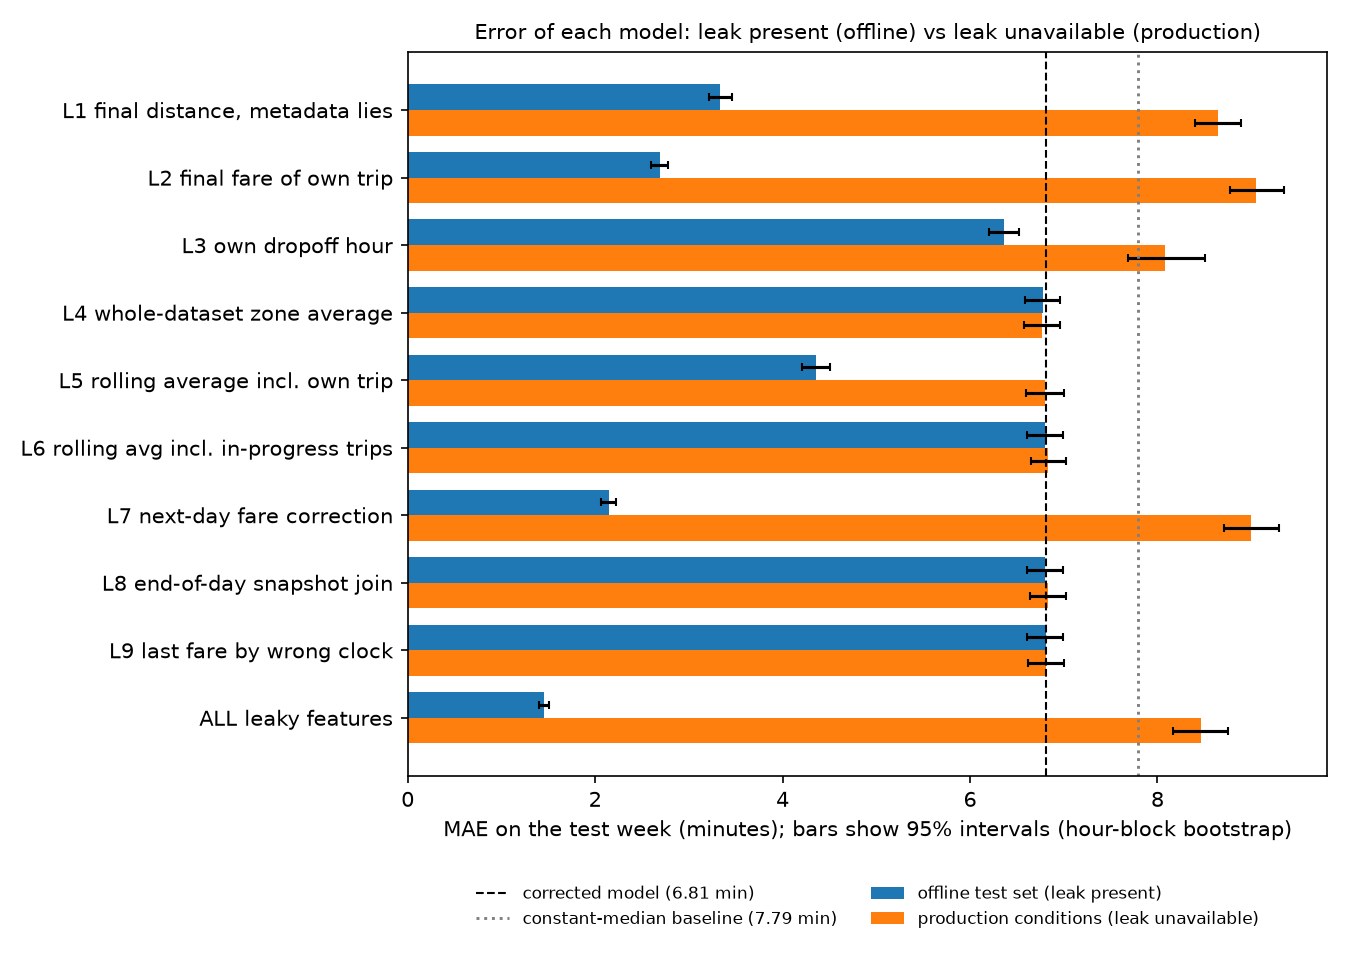
\includegraphics[width=0.92\linewidth,trim=0 0 0 21.1bp,clip]{fig_offline_vs_production.png}
\caption{Offline versus production-condition MAE for each leaky model.}
\label{fig:offprod}
\end{figure}

\paragraph{The share of flagged rows does not predict the damage.} \autoref{fig:flagged} plots, for every leaky feature, the share of examples the auditor flagged (horizontal axis) against the change in offline MAE relative to the honest model (vertical axis; negative means lower error). If the flagged share predicted the damage, the points would line up along a rising curve; instead seven leaky features sit at 100\% of rows with effects from $-0.3\%$ (L8) to $-68.4\%$ (L7), and L6 (98.2\%) and L9 (90.3\%) change the score by $0.2\%$ or less. The flagged share measures how often a rule is violated, not how informative the leaked value is. Four of these leaks (L4, L6, L8, L9) move the MAE by 0.051 min or less; a score-based check would not notice them, but the availability audit flags all four. This is the main argument for auditing availability rather than watching metrics.

In \autoref{fig:flagged} the horizontal axis starts at 86\% so that L9 (90.3\%) and L6 (98.2\%) can be told apart from the features at 100\%. Seven points form a column at 100\%: L7 ($-68.4\%$), L2 ($-60.3\%$), L1 ($-51.1\%$), L5 ($-35.9\%$), L3 ($-6.6\%$), L4 ($-0.8\%$) and L8 ($-0.3\%$). The two points left of the column, L6 and L9, are both within 0.2\% of zero. The four points near zero (L4, L6, L8, L9) lie below the 0.066 min float-level jitter measured in \autoref{sec:sens}, so their order in \autoref{fig:flagged} is not meaningful.

\begin{figure}[H]
\centering
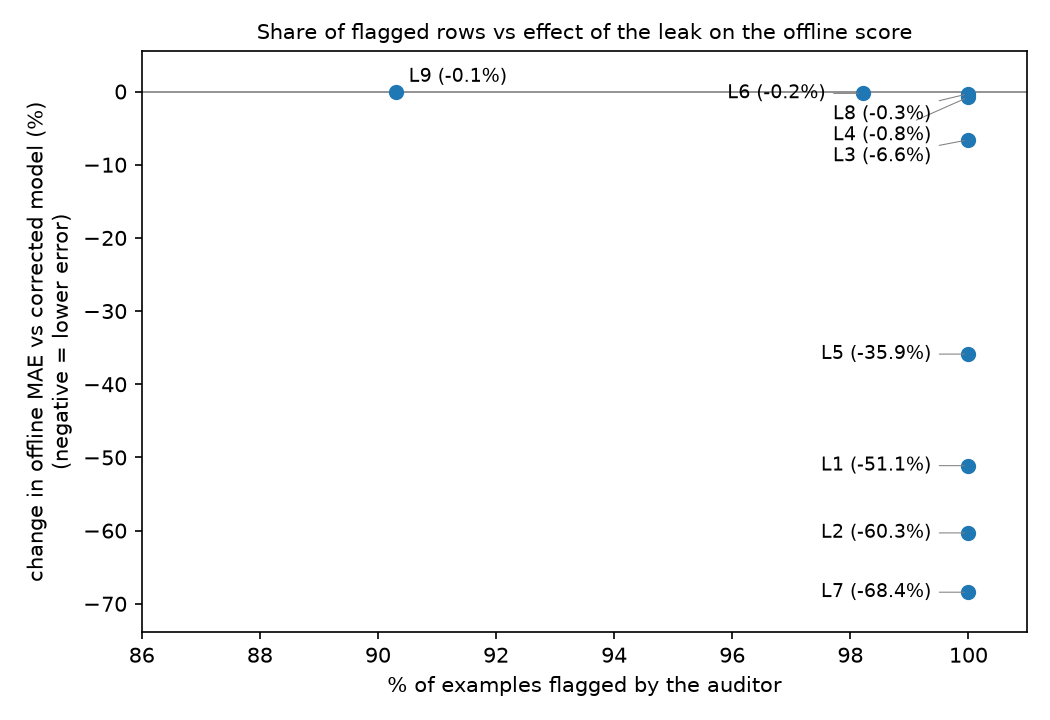
\includegraphics[width=0.78\linewidth,trim=0 0 0 21.1bp,clip]{fig_flagged_vs_effect.png}
\caption{Share of examples flagged versus effect on offline MAE.}
\label{fig:flagged}
\end{figure}

\paragraph{Low correlation does not mean safe.} The dropoff hour (L3) has a correlation of 0.001 with the target on its own, yet adding it lowers the offline MAE by 6.6\%, because together with pickup hour it reveals the trip's length at hour resolution. Likewise the safe 60-minute average (N5) correlates 0.541 with the target, the version including the own trip (L5) 0.617, and the in-progress version (L6) 0.566; a whole-dataset zone average (L4, 0.535) is almost indistinguishable from its safe counterpart (0.534), because aggregates that pool about $10^4$ trips barely change when a few future trips are included. Leakage magnitude grows as the aggregated group shrinks: L4 is real but nearly invisible to metrics.

\subsection{Production conditions: the gain disappears or reverses}\label{sec:prod}
\begin{table}[H]
\centering\small
\caption{Production-condition MAE and paired difference.}
\label{tab:prod}
\begin{tabular}{@{}l r r r l@{}}
\toprule
Model & Offline MAE & Production MAE & Prod.\ $-$ corrected [95\% CI] & Verdict \\
\midrule
+ L1 distance & 3.332 & 8.626 & $+1.808$ [$+1.678$, $+1.940$] & worse \\
+ L2 total amount & 2.706 & 9.075 & $+2.257$ [$+2.103$, $+2.408$] & worse \\
+ L3 dropoff hour & 6.368 & 7.912 & $+1.095$ [$+0.773$, $+1.482$] & worse \\
+ L4 global zone avg & 6.766 & 6.762 & $-0.055$ [$-0.075$, $-0.036$] & better \\
+ L5 60\,min self & 4.372 & 6.806 & $-0.012$ [$-0.052$, $+0.030$] & no clear diff. \\
+ L6 in-progress & 6.801 & 6.842 & $+0.025$ [$+0.002$, $+0.046$] & worse \\
+ L7 fare correction & 2.153 & 9.035 & $+2.218$ [$+2.076$, $+2.358$] & worse \\
+ L8 snapshot & 6.797 & 6.822 & $+0.004$ [$-0.017$, $+0.026$] & no clear diff. \\
+ L9 last fare & 6.811 & 6.809 & $-0.008$ [$-0.025$, $+0.008$] & no clear diff. \\
+ ALL leaky & 1.451 & 8.471 & $+1.653$ [$+1.513$, $+1.789$] & worse \\
\bottomrule
\end{tabular}
\end{table}

\autoref{tab:prod} replaces the leaked value by what is available at prediction time and gives the difference to the corrected model (6.817 min) with its 95\% interval; ``worse'' means the interval lies entirely above zero and ``better'' entirely below. Together with \autoref{fig:offprod} it shows that models relying on a value that does not yet exist (L1, L2, L7 and the all-leaks model) are 24\% to 33\% \emph{worse} than the honest model once the leak is gone (MAE 8.47 to 9.08 against 6.817), and above the constant-median baseline of 7.787; their production error is 2.6 to 5.8 times their offline error. L5's offline gain of $-35.9\%$ disappears completely in production ($-0.012$ min, no clear difference): it was inflation only. L4 is slightly \emph{better} than the honest model in production ($-0.055$ min, about 3 seconds); an untested explanation is that the whole-month zone average is a steadier training feature than the as-of one. This does not make L4 acceptable, since it still uses information from after \tpred{}. Verdicts near zero (L4, L5, L6, L8, L9) are not resolved by these intervals; \autoref{sec:sens} explains why. The comparison with the baseline is made by eye against a point value; the baseline's own uncertainty is not drawn.

\subsection{Ablations}
\begin{table}[H]
\centering\small
\caption{Ablation results.}
\label{tab:abl}
\begin{tabular}{@{}l r r r r r@{}}
\toprule
Ablation & Without & With & $\Delta$MAE [95\% CI] & $\Delta$\% & Full exp. \\
\midrule
L5 without N5 & 6.797 & 6.586 & $-0.212$ [$-0.256$, $-0.169$] & $-3.1$ & $-35.9$ \\
L3 without \ft{pickup_hour} & 6.962 & 6.841 & $-0.121$ [$-0.159$, $-0.085$] & $-1.7$ & $-6.6$ \\
\bottomrule
\end{tabular}
\end{table}

Each row of \autoref{tab:abl} compares two models that both lack the helper feature (N5 or \ft{pickup_hour}), with and without the leak; the last column repeats the leak's effect in the full experiment. \autoref{tab:abl} supports the first hypothesis: L5's gain shrinks about twelve-fold without N5, so the model recovers the target from the safe average and the average that additionally contains the trip's own duration. L3's gain shrinks about four-fold without pickup hour; the remaining $-1.7\%$ is plausibly the dropoff hour acting as a proxy for the missing pickup hour, which was not tested. Removing N5 from the corrected model changed its MAE from 6.817 to 6.797 (not tested for significance), so N5 appears redundant for the honest model.

\subsection{Float-level feature noise}\label{sec:sens}
\begin{table}[H]
\centering\footnotesize
\caption{Float-noise study: spread of MAE over 20 refits.}
\label{tab:sens}
\begin{tabular}{@{}l r r r r r r l@{}}
\toprule
Model & Ref.\ MAE & SD & Min--max & Effect & Paired SD & Lower & Reading \\
\midrule
corrected & 6.817 & 0.0073 & 6.778--6.808 & (ref.) & & & \\
+ L1 & 3.332 & 0.0050 & 3.317--3.339 & $-3.469$ & 0.0102 & 20/20 & clear \\
+ L2 & 2.706 & 0.0139 & 2.673--2.716 & $-4.106$ & 0.0177 & 20/20 & clear \\
+ L3 & 6.368 & 0.0089 & 6.361--6.391 & $-0.426$ & 0.0131 & 20/20 & clear \\
+ L4 & 6.766 & 0.0098 & 6.755--6.791 & $-0.029$ & 0.0128 & 20/20 & borderline \\
+ L5 & 4.372 & 0.0181 & 4.332--4.397 & $-2.438$ & 0.0182 & 20/20 & clear \\
+ L6 & 6.801 & 0.0071 & 6.789--6.822 & $+0.006$ & 0.0120 & 5/20 & not distinct \\
+ L7 & 2.153 & 0.0029 & 2.133--2.147 & $-4.661$ & 0.0077 & 20/20 & clear \\
+ L8 & 6.797 & 0.0100 & 6.773--6.807 & $-0.008$ & 0.0129 & 13/20 & not distinct \\
+ L9 & 6.811 & 0.0047 & 6.813--6.826 & $+0.020$ & 0.0097 & 0/20 & borderline (higher) \\
+ ALL & 1.451 & 0.0053 & 1.443--1.463 & $-5.344$ & 0.0086 & 20/20 & clear \\
\bottomrule
\end{tabular}
\end{table}

Rebuilding the database once changed some feature values at the $10^{-13}$ level, caused by order-dependent float sums over tied timestamps, and moved the L6 offline MAE from 6.804 to 6.796. Although the build is now deterministic, the same noise could come from another platform or library version. In \autoref{tab:sens}, SD and min--max describe one model's MAE across the 20 refits, the effect is the mean paired difference to the corrected model, and ``Lower'' counts the refits in which the leaky model beats the corrected one. The table shows that one model's MAE has a standard deviation of 0.003 to 0.018 min under such noise, with a largest min--max spread of 0.066 min (L5). Differences between models of that order are not interpretable. A larger noise ($10^{-9}$, 10 refits, recorded in the project log but not kept as a result file) gave a similar spread, which suggests the sensitivity comes from tie-breaking in the model's histogram bins rather than the noise size; this is a hypothesis, not a result.

\emph{Reading rule} (applied in the last column of \autoref{tab:sens}; chosen by the author, not a statistical test): an effect counts only if its sign is the same in at least 90\% of the refits; it is \emph{clear} if the mean effect is at least ten times the paired SD, \emph{borderline} if two to ten times, and otherwise not distinguishable from zero. L4 (ratio 2.25) and L9 (2.01) sit close to the threshold and should not be over-interpreted. L9 shows a consistent small \emph{increase} in error (0 of 30 refits lower across both noise levels) that the bootstrap, which covers test sampling only, could not reveal. The reported MAE of the unperturbed build lies outside the refits' min--max range for 3 of 11 models (corrected, L7, L9); the cause was not investigated. The study covers \emph{offline} scores only: production verdicts close to zero (L4, L5, L6, L8, L9) remain unresolved, while the production effects of L1, L2, L3, L7 and ALL ($+1.1$ to $+2.3$ min) are tens of times the jitter.

\paragraph{How to quote the numbers.} The honest model scores 6.817 min (jitter SD 0.007), and differences below 0.066 min should not be interpreted.

\subsection{Performance}
\begin{table}[H]
\centering\scriptsize\setlength{\tabcolsep}{3pt}
\caption{Runtime and peak memory by data size.}
\label{tab:bench}
\begin{tabular}{@{}r r r r r r r r@{}}
\toprule
Examples & Trips & Pipeline s & Audit s & ML s & Total s & Peak MiB & First run s \\
\midrule
10{,}000 & 19{,}928 & 1.6 (1.6--1.7) & 1.1 (1.1--1.2) & 21.9 (21.6--22.0) & 24.7 (24.4--24.7) & 226 (226--226) & 24.4 \\
50{,}000 & 99{,}640 & 3.6 (3.6--3.6) & 2.1 (2.1--2.1) & 32.5 (32.2--35.3) & 38.2 (37.9--41.0) & 264 (264--265) & 37.9 \\
200{,}000 & 398{,}557 & 6.8 (6.7--6.8) & 5.0 (5.0--5.3) & 73.9 (73.5--75.1) & 85.7 (85.5--86.8) & 434 (425--434) & 85.5 \\
\bottomrule
\end{tabular}
\end{table}

The full workflow runs on a 4~GB laptop (\autoref{tab:bench}; cells show the median of three runs with the min--max in parentheses, and ``first run'' is the total time of the first repetition). ML (the 11 experiments, the same 11 again for the production analysis, and the ablation fits, with 500 bootstrap resamples) takes 85\% to 89\% of the total time. A twenty-fold increase in examples gives 3.5 times the total time and 1.9 times the peak memory. The first run was not slower than the median at any size, so no cold-start penalty is visible; ``cold'' here means a fresh process, because the operating system's file cache was not cleared. Peak memory is the peak working set of the measured process over the whole run; data generation is not included. These timings are not comparable with the real-data pipeline timings in the project log (29.4 s for 2.9 million trips and 100{,}000 examples), which use a different data set (258 pickup zones instead of 60) and size definition.

\section{Discussion and Limitations}\label{sec:limits}
\subsection{What the results support}
Three observations hold in this setting. First, an availability audit finds leaks that scores cannot: four leaks move the MAE by at most 0.051 min and are flagged by the auditor anyway. Second, the impression of damage in offline scores depends on how informative the leaked value is, not on how often a rule is violated. Third, offline gains from leaks can vanish or reverse in production, up to 33\% worse than the honest model when a value that does not yet exist is missing at serving time.

\subsection{Three sources of uncertainty}
Every MAE in this report is uncertain in at least three ways, and only the first two were measured. (1)~\emph{Test sampling}: the intervals in \autoref{tab:offline} to \autoref{tab:abl} come from an hour-block bootstrap of one test week. (2)~\emph{Float-level feature noise}: measured separately, for offline scores only. (3)~\emph{Not studied}: other chronological splits, other months, other model seeds and model classes, and real rather than simulated availability lags. The bootstrap intervals describe the first source only, so the full uncertainty is wider than they suggest, and the bootstrap by hour does not capture day-level variation (only seven test days).

\subsection{Limitations}
\begin{itemize}
  \item \textbf{Availability times are simulated} from configurable lags, not observed. Results such as the share of rows flagged for L9 depend on them. A sensitivity analysis over the lags (0, 2 and 5 minutes) is planned but not done.
  \item \textbf{Scenarios and auditor were designed together.} A perfect score shows agreement with the specification, not general leakage detection; the auditor reports explicit rule violations only.
  \item \textbf{R4 supports duration aggregates grouped by zone.} Other aggregates raise an error, and the conformance check covers six aggregates. A false declaration for an aggregate outside this list would be missed.
  \item \textbf{One month, one chronological split (last 7 days), one model class.} Trips of 1 to 180 minutes only.
  \item \textbf{Production conditions are a simulation}, with serving values chosen by the author.
  \item \textbf{Synthetic benchmark data} has 60 zones, so its lookback windows pool more trips than on the real data.
  \item \textbf{Several explanations are untested hypotheses}: why L4 is slightly better in production, why the float-noise spread does not depend on the noise size, and why 3 of 11 unperturbed MAEs lie outside the refit ranges.
\end{itemize}

\subsection{A defect found by checking reproducibility}\label{sec:defect}
Comparing two rebuilds of the database showed that feature values differed at the $10^{-13}$ level, enough to change a model score in the third decimal (largest shift in any offline MAE: 0.0157 min). The cause was diagnosed as order-dependent float sums over rows with tied timestamps; the fix (accumulating integer seconds) and a regression test make rebuilds identical, and two Windows rebuilds and a Windows--Ubuntu comparison of the demo agreed to $10^{-9}$ in every column. The diagnosis is supported by the fix and the test but was not traced inside DuckDB. An earlier claim that offline MAEs reproduced to $10^{-9}$ was also corrected: it had only compared refits on one database, not rebuilds. Documenting this matters because the shift was larger than several effects the project reports.

\section{Conclusion and Future Work}\label{sec:future}
LeakScope turns the question ``was this value usable at prediction time?'' into rules that can be run, explained and tested at boundary cases, and a controlled study shows why such an audit is needed: leaks can produce scores that look excellent offline, can be nearly invisible in the metric, and can fail in production. The conclusions are limited by simulated availability, co-designed scenarios and a single month, split and model class.

Planned and not done: sensitivity of all results to the simulated availability lags (0, 2 and 5 minutes); feature dependency analysis; a comparison with an existing feature-serving system; production-condition sensitivity to noise; other splits, months and model seeds; and support for aggregates beyond duration by zone.

\section{Reproducibility}
The code, configuration, tests and generated report are in the repository \url{https://github.com/0utc/leakscope}. A one-command demo needs no download (\ft{python -m leakscope demo}); it uses synthetic data and is not comparable with the real-data numbers above. The real-data numbers come from Python 3.13.11, scikit-learn 1.9.1, DuckDB 2.0.0 on Windows 11 with seed 0; dependency versions are not pinned in the project, so another install may differ. The real-data results are reproduced, in order, by:
\begin{verbatim}
python -m leakscope pipeline
python -m leakscope audit
python -m leakscope experiment
python -m leakscope sensitivity
python -m leakscope benchmark
python -m leakscope report
\end{verbatim}
The test suite (\ft{pytest}) ran 102 passed and 9 skipped on a clean clone (the skipped tests need the real database), and CI runs on Ubuntu and Windows with Python 3.11 and 3.13.

\clearpage
\appendix
\section{Feature registry}
\autoref{tab:registry} lists every registered feature with its kind, scenario, availability clock and window.

\begin{table}[H]
\centering\scriptsize
\caption{Registered features.}
\label{tab:registry}
\begin{tabular}{@{}l l l l l@{}}
\toprule
Feature & Kind & Scen. & Availability clock & Window \\
\midrule
\ft{pickup_hour}, \ft{pickup_dow} & row & N1 & avail\_pickup & --- \\
\ft{pu_zone} & row & N1 & avail\_pickup & --- \\
\ft{passenger_count_filled}, \ft{passenger_missing} & row & N1 & avail\_pickup & --- \\
\ft{zone_avg_dur_asof} & aggregate & N2 & avail\_dropoff & up to \tpred{} \\
\ft{zone_avg_dur_7d} & aggregate & N3 & avail\_dropoff & 7 days \\
\ft{zone_avg_dur_60m} & aggregate & N5 & avail\_dropoff & 60 min \\
\ft{leak_trip_distance} & row & L1 & avail\_pickup (false) & --- \\
\ft{leak_total_amount} & row & L2 & avail\_fare & --- \\
\ft{leak_dropoff_hour} & row & L3 & avail\_dropoff & --- \\
\ft{leak_zone_avg_global} & aggregate & L4 & avail\_dropoff & whole dataset \\
\ft{leak_zone_avg_60m_self} & aggregate & L5 & avail\_dropoff & 60 min, incl.\ own \\
\ft{leak_zone_avg_60m_inprogress} & aggregate & L6 & avail\_dropoff & 60 min by pickup \\
\ft{leak_fare_correction} & row & L7 & avail\_fare\_correction & --- \\
\ft{leak_snapshot_zone_avg} & row & L8 & avail\_snapshot\_eod & --- \\
\ft{leak_last_fare_zone} & row (lookup) & L9 & avail\_fare & --- \\
\bottomrule
\end{tabular}
\end{table}

\section{Simulated availability lags}
\autoref{tab:lags} gives the simulated availability rules behind every result; they are assumptions and are configurable.

\begin{table}[H]
\centering\small
\caption{Simulated availability lags.}
\label{tab:lags}
\begin{tabular}{@{}l l@{}}
\toprule
Field & Availability \\
\midrule
Pickup time, zone, passengers & at pickup (lag 0) \\
Dropoff time, duration & at dropoff (+0 min) \\
Final trip distance & at dropoff (+0 min) \\
Final fare, total amount & dropoff + 2 min \\
Fare correction & 06:00 on the day after dropoff \\
Zone aggregate & latest availability among its source trips \\
\bottomrule
\end{tabular}
\end{table}

\clearpage
\phantomsection
\addcontentsline{toc}{section}{References}
\bibliographystyle{plainnat}
\bibliography{references}

\end{document}
